\documentclass{article}\usepackage[]{graphicx}\usepackage[]{color}
%% maxwidth is the original width if it is less than linewidth
%% otherwise use linewidth (to make sure the graphics do not exceed the margin)
\makeatletter
\def\maxwidth{ %
  \ifdim\Gin@nat@width>\linewidth
    \linewidth
  \else
    \Gin@nat@width
  \fi
}
\makeatother

\definecolor{fgcolor}{rgb}{0.345, 0.345, 0.345}
\newcommand{\hlnum}[1]{\textcolor[rgb]{0.686,0.059,0.569}{#1}}%
\newcommand{\hlstr}[1]{\textcolor[rgb]{0.192,0.494,0.8}{#1}}%
\newcommand{\hlcom}[1]{\textcolor[rgb]{0.678,0.584,0.686}{\textit{#1}}}%
\newcommand{\hlopt}[1]{\textcolor[rgb]{0,0,0}{#1}}%
\newcommand{\hlstd}[1]{\textcolor[rgb]{0.345,0.345,0.345}{#1}}%
\newcommand{\hlkwa}[1]{\textcolor[rgb]{0.161,0.373,0.58}{\textbf{#1}}}%
\newcommand{\hlkwb}[1]{\textcolor[rgb]{0.69,0.353,0.396}{#1}}%
\newcommand{\hlkwc}[1]{\textcolor[rgb]{0.333,0.667,0.333}{#1}}%
\newcommand{\hlkwd}[1]{\textcolor[rgb]{0.737,0.353,0.396}{\textbf{#1}}}%
\let\hlipl\hlkwb

\usepackage{framed}
\makeatletter
\newenvironment{kframe}{%
 \def\at@end@of@kframe{}%
 \ifinner\ifhmode%
  \def\at@end@of@kframe{\end{minipage}}%
  \begin{minipage}{\columnwidth}%
 \fi\fi%
 \def\FrameCommand##1{\hskip\@totalleftmargin \hskip-\fboxsep
 \colorbox{shadecolor}{##1}\hskip-\fboxsep
     % There is no \\@totalrightmargin, so:
     \hskip-\linewidth \hskip-\@totalleftmargin \hskip\columnwidth}%
 \MakeFramed {\advance\hsize-\width
   \@totalleftmargin\z@ \linewidth\hsize
   \@setminipage}}%
 {\par\unskip\endMakeFramed%
 \at@end@of@kframe}
\makeatother

\definecolor{shadecolor}{rgb}{.97, .97, .97}
\definecolor{messagecolor}{rgb}{0, 0, 0}
\definecolor{warningcolor}{rgb}{1, 0, 1}
\definecolor{errorcolor}{rgb}{1, 0, 0}
\newenvironment{knitrout}{}{} % an empty environment to be redefined in TeX

\usepackage{alltt}
\usepackage{amsmath}
\usepackage{enumitem}
\usepackage{ amssymb }
\usepackage{ textcomp }
\usepackage{ dsfont }
\usepackage{mathtools}
\usepackage{caption}

\topmargin=-0.5in
\evensidemargin=0in
\oddsidemargin=0in
\textwidth=6.5in
\textheight=9.0in
\headsep=0.25in

\DeclarePairedDelimiter{\abs}{\lvert}{\rvert}

\title{diffloop: analysis of variable loops under different models}
\author{Caleb Lareau and Martin Aryee}
\date{\today}
\IfFileExists{upquote.sty}{\usepackage{upquote}}{}
\begin{document}
\maketitle
\captionsetup[figure]{labelformat=empty}

\section*{Overview}
The purpose of this document is to provide a high-level comparison of different models fit to the K562 and MCF7 ChIA-PET data from ENCODE. Specifically, we examine the association statistics from using voom, edgeR, and binned associations. 

\section*{Mean-Variance Plot}
The mean-variance plot of the ChIA-PET data analyzed in this manuscript is shown in \textbf{Figure S1}. RNA-Seq count data is often modeled as negative binomial, since the variance exceeds the mean resulting in an overdispersion relative to the Poisson model. We hypothesized that a similar model could be applied to counts data in the diffloop framework. 

\begin{figure}[h]
\begin{knitrout}
\definecolor{shadecolor}{rgb}{0.969, 0.969, 0.969}\color{fgcolor}

{\centering 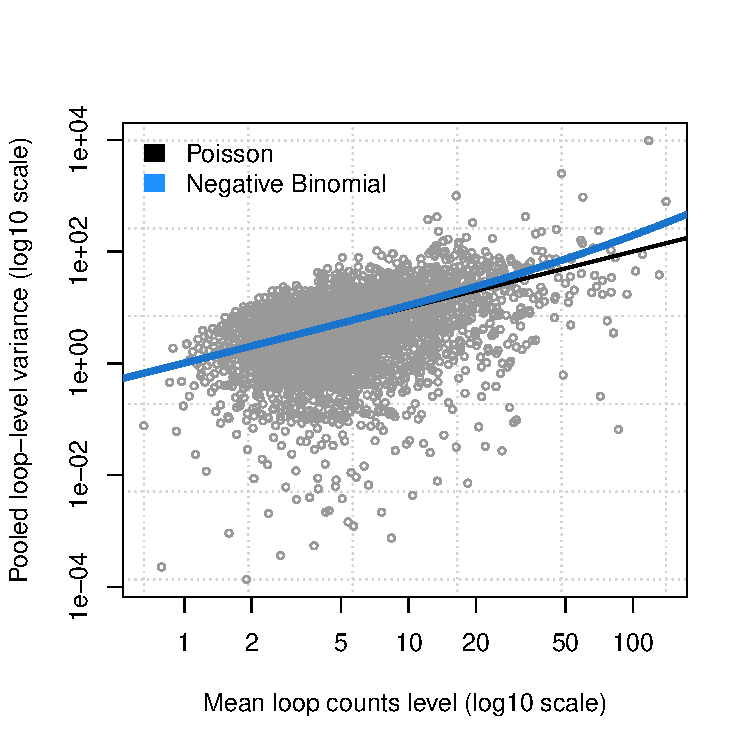
\includegraphics[width=\maxwidth]{figure/mvPlot-1} 

}



\end{knitrout}
\centering
\caption{\textbf{Figure S1.} Mean-variance plot of 2x2 differential association between MCF7 and K562.}
\end{figure} \newpage

While the Negative Binomial line does not obviously deviate from the Poisson line for the loop counts data considered here, we note a similar pattern in RNA-Seq data for low counts in the displayed range while the variance deviates more clearly from the mean at larger count values. We expect that similar behaviour will be observed at higher ChIA-PET counts and therefore implemented the negative binomial as the default model in diffloop. 


\section*{Loop Width Stratification}
Though the size factor correction as implemented in diffloop adjusts for variable read depth between samples (Figure 2), we considered whether or not the size factor should vary with the loop width spanning the two anchors. For example, the plot below of differential associations calculated within loop width strata shows a potential weak dependence on loop width (\textbf{Figure S2}). 

\begin{figure}[h]
\begin{knitrout}
\definecolor{shadecolor}{rgb}{0.969, 0.969, 0.969}\color{fgcolor}

{\centering 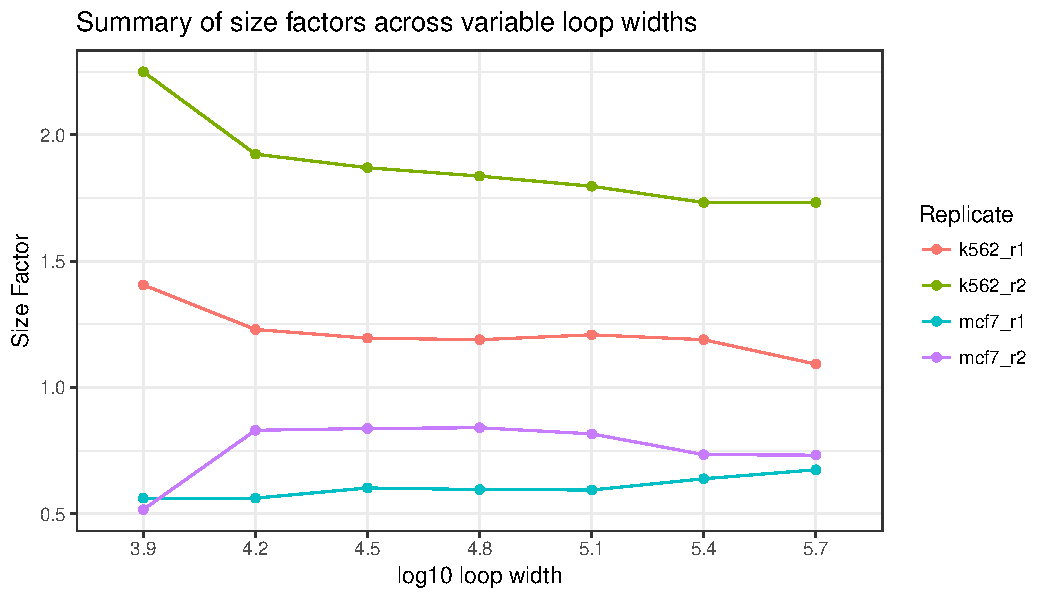
\includegraphics[width=\maxwidth]{figure/linePlot-1} 

}



\end{knitrout}
\centering
\caption{\textbf{Figure S2.} Variable size factor across different loop widths (distance spanned between the midpoint of the anchors).}
\end{figure}

To assess the effect of variable loop widths, we binned loops based on their distance spanned using the groups above (increments of 0.3 on the $\log_{10}$ scale) and assessed differential looping within each stratum individually. \textbf{Figure S3} shows a per-loop comparison of the $-\log_{10}$ ratio of the q-values using the standard model compared to the stratified model. Loops annotated in red and blue are shown with summary statistics in \textbf{Table S1} and \textbf{Table S2}.

\begin{figure}[h]
\begin{knitrout}
\definecolor{shadecolor}{rgb}{0.969, 0.969, 0.969}\color{fgcolor}

{\centering 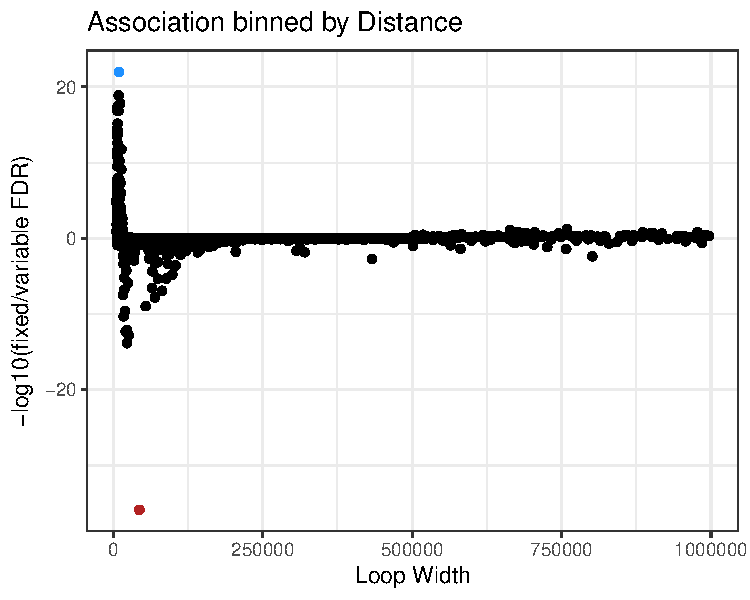
\includegraphics[width=\maxwidth]{figure/other-1} 

}



\end{knitrout}
\centering
\caption{\textbf{Figure S3.} Comparison of per-loop statistical significance with using the standard unstratified model vs. a stratified model based on loop width. Loops marked in red are more significant ($> 20$ orders of magnitude) when using the unstratified model between the tests whereas the blue loops are more significant ($>20$ orders of magnitude) when using the stratified model. The Y axis shows the $-\log_{10}$ ratio of the q-values. \newline}
\end{figure} \newpage \newpage 

\begin{figure}[h]
\begin{knitrout}
\definecolor{shadecolor}{rgb}{0.969, 0.969, 0.969}\color{fgcolor}
\begin{tabular}{l|l|l|l|l|l|l}
\hline
k562\_r1 & k562\_r2 & mcf7\_r1 & mcf7\_r2 & LoopWidth & Regular.FDR & Variable.SF.FDR\\
\hline
9 & 19 & 158 & 194 & 43600 & 1.07e-64 & 1.37e-104\\
\hline
\end{tabular}


\end{knitrout}
\centering
\caption{\textbf{Table S1.} Summary statistics of the loops marked in red in \textbf{Figure S3.} These loops were highlighted due to large differences in the summary statistic measures such that the unstratified model yielded a less significant test statistic. Individual replicate PET counts, the distance the loop spans, as well as the q-values for each test are displayed. \newline } 
\end{figure}

\begin{figure}[h]
\begin{knitrout}
\definecolor{shadecolor}{rgb}{0.969, 0.969, 0.969}\color{fgcolor}
\begin{tabular}{l|l|l|l|l|l|l}
\hline
k562\_r1 & k562\_r2 & mcf7\_r1 & mcf7\_r2 & LoopWidth & Regular.FDR & Variable.SF.FDR\\
\hline
0 & 0 & 75 & 114 & 9360 & 1.3e-61 & 7.12e-43\\
\hline
\end{tabular}


\end{knitrout}
\centering
\caption{\textbf{Table S2.} Summary statistics of the loops marked in blue in \textbf{Figure S3.} These loops were highlighted due to large differences in the summary statistic measures such that the unstratified model yielded a more significant test statistic. Individual replicate PET counts, the distance the loop spans, as well as the q-values for each test are displayed.}
\end{figure}  \clearpage

We note that all the highlighted loops are deeemed highly statistically significant in both stratified and unstratified analyses. To explore whether the two models identify different sets of differential loops we plotted the $-\log_{10}$ q-values against each other after applying a ceiling of 4 (q = 0.0001) (\textbf{Figure S4}). Of note, few loops tended to deviate significantly in this range indicating that either approach produces a very similar set of differential loops. Thus, in the present implementation of diffloop, a single unstratified model is applied and the loop width is not considered. As more topology libraries become available, novel methods of association, including those that account for loop width, may be incorporated in the package as the evidence demands.  

\begin{figure}[h]
\begin{knitrout}
\definecolor{shadecolor}{rgb}{0.969, 0.969, 0.969}\color{fgcolor}

{\centering 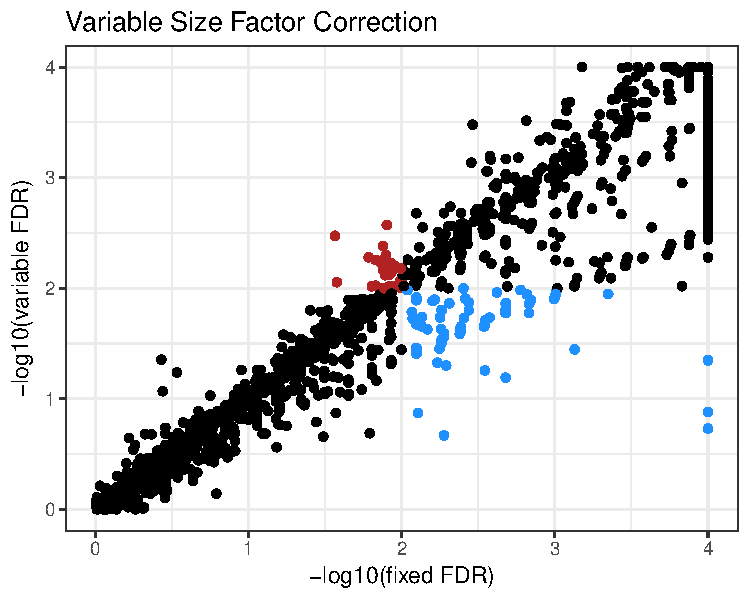
\includegraphics[width=\maxwidth]{figure/closeMDF-1} 

}



\end{knitrout}
\centering
\caption{\textbf{Figure S4.} A scatter plot comparing the $-\log_{10}$ FDR q-values between 0 and 4 of the fixed and binned association tests. For either test, $-\log_{10}$ FDR q-values greater than 4 were shrunk to 4 for visualization. Loops marked in red were differential (q-value $<0.01$) in the binned association test.} 
\end{figure}  \clearpage


\section*{Comparison with Voom}
As an alternative model to Negative Binomial regression for RNA-Seq data, the limma-voom method approximates the mean-variance relationship of the log-counts and applies a moderated t-test. We implemented a similar approach for finding differential loops analogous to differential transcripts in this model. \textbf{Figure S5} shows a per-loop comparison of the Negative Binomial regression (edgeR) and the voom q-values as a function of loop width. We also highlight the largest deviants in \textbf{Table S3}. 

\begin{figure}[h]
\begin{knitrout}
\definecolor{shadecolor}{rgb}{0.969, 0.969, 0.969}\color{fgcolor}

{\centering 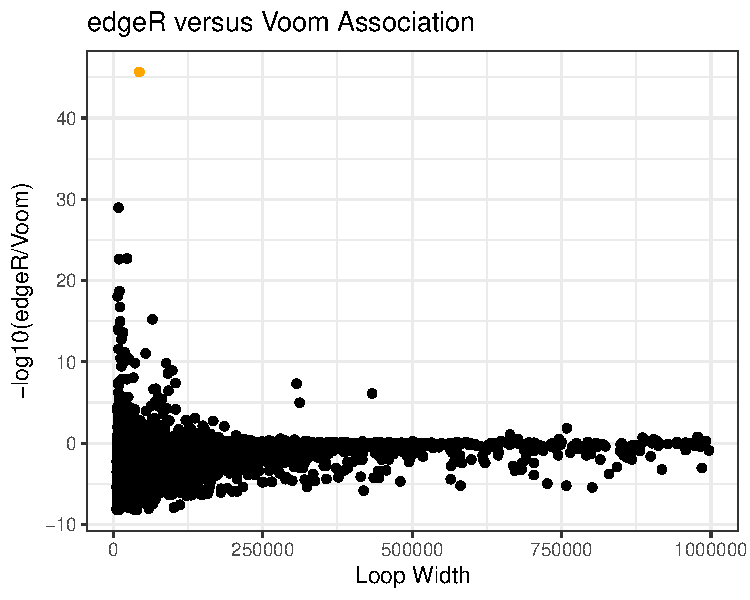
\includegraphics[width=\maxwidth]{figure/evv-1} 

}



\end{knitrout}
\centering
\caption{\textbf{Figure S5.} Comparison of per-loop statistical significance using models from edgeR and Voom. Loops highlighted in orange were assigned a much more statistically significant q-value in edgeR ($> 30$ orders of magnitude) than voom. These loops are shown in \textbf{Table S3}.}
\end{figure}

\begin{figure}[h]
\begin{knitrout}
\definecolor{shadecolor}{rgb}{0.969, 0.969, 0.969}\color{fgcolor}
\begin{tabular}{l|l|l|l|l|l|l}
\hline
k562\_r1 & k562\_r2 & mcf7\_r1 & mcf7\_r2 & LoopWidth & edgeR.FDR & Voom.FDR\\
\hline
9 & 19 & 158 & 194 & 43600 & 1.07e-64 & 4.78e-19\\
\hline
\end{tabular}


\end{knitrout}
\centering
\caption{\textbf{Table S3.} Summary statistics of the loops marked in orange in \textbf{Figure S5.} These loops were highlighted due to large differences ($> 30$ orders of magnitude) in the summary statistic measures between the edgeR and Voom association models.}
\end{figure}  \clearpage 

A trend emerges as shown in \textbf{Figure S5} where differential loops spanning smaller distances were more statistically significant in the edgeR association model. We note however that the loops with the largest deviation (orange, \textbf{Table S4}) are in fact highly significant in both models. To assess whether any loops might switch from 'significant' to 'not significant' we again plotted the $-\log_{10}$ q-values with a cap at 4 (\textbf{Figure S6}). Loops that are significant in one model but not the other are marked by color. Summary statistics for the orange loops, where edgeR indicates a highly significancant difference (FDR $< 0.01$) whereas voom suggests no/little difference (FDR $> 0.1$) are shown in \textbf{Table S4}. 

\begin{figure}[h]
\begin{knitrout}
\definecolor{shadecolor}{rgb}{0.969, 0.969, 0.969}\color{fgcolor}

{\centering 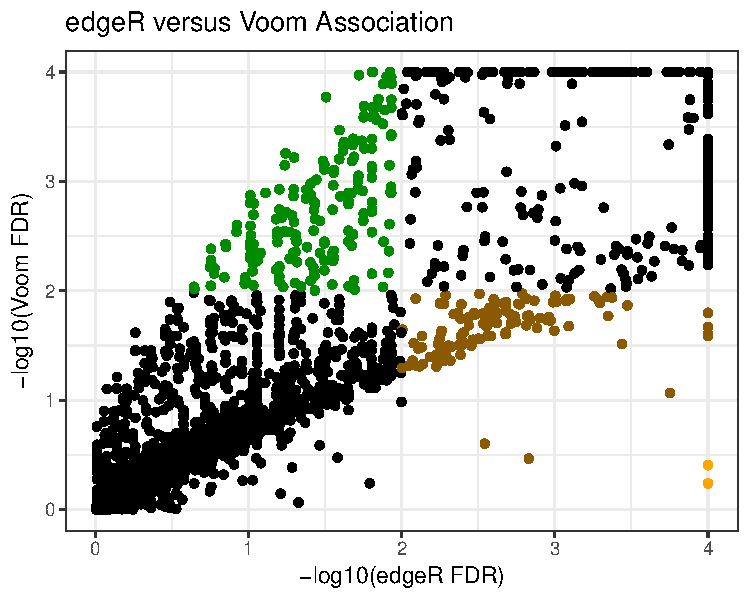
\includegraphics[width=\maxwidth]{figure/closeMDFvoom-1} 

}



\end{knitrout}
\centering
\caption{\textbf{Figure S6.} Comparison of per-loop statistical significance using models from edgeR and voom. Loops highlighted in orange were indicated as the edgeR model provided more statistically significant FDR value. These loops are shown in \textbf{Table S4}.}
\end{figure}


\begin{figure}[h]
\begin{knitrout}
\definecolor{shadecolor}{rgb}{0.969, 0.969, 0.969}\color{fgcolor}
\begin{tabular}{l|l|l|l|l|l|l}
\hline
k562\_r1 & k562\_r2 & mcf7\_r1 & mcf7\_r2 & LoopWidth & edgeR.FDR & Voom.FDR\\
\hline
165 & 61 & 7 & 12 & 8600 & 3.1e-15 & 0.393\\
\hline
2 & 1 & 0 & 50 & 65500 & 3.44e-16 & 0.576\\
\hline
\end{tabular}


\end{knitrout}
\centering
\caption{\textbf{Table S4.} Summary statistics of the loops marked in orange in \textbf{Figure S6.} These loops were highlighted due to differences in the summary statistic measures such that they were differential (FDR $< 0.01$) in the edgeR model but not differential (FDR $> 0.1$) in the voom model.}
\end{figure} \clearpage

\end{document}

